\chapter{Auswertung Projektplan} \label{appendix:sprints}

In diesem Kapitel wird die Planung der einzelnen Phasen und insbesondere der Sprints in der Construction-Phase mit der Realität verglichen. Es wird jeweils aufgezeigt, was die Ziele, Probleme und erreichten Punkte waren sowie ein Vergleich der geplanten und tatsächlich benötigten Punkte.

\subimport{}{inception.tex}
\subimport{}{elaboration.tex}
\subimport{}{sprint-1.tex}
\subimport{}{sprint-2.tex}
\subimport{}{sprint-3.tex}
\subimport{}{sprint-4.tex}
\subimport{}{sprint-5.tex}
\subimport{}{transition.tex}

\section*{Total und Fazit}

\xxx[Daten eintragen]

\begin{table}[H]
	\centering
	\begin{tabular}{ll}
		\toprule
		\multicolumn{2}{l}{\textbf{Total}}\\
		\midrule
		\textbf{Periode} & 22.02.2016\textendash 17.06.2016\\
		\textbf{Stunden Soll} & \SI{720}{\hour}\\
		\textbf{Stunden Ist} & \SI{763}{\hour}\\
		\bottomrule
	\end{tabular}
\end{table}

\begin{table}[H]
	\centering
	\begin{tabular}{ll}
		\toprule
		\multicolumn{2}{l}{\textbf{Total pro Person}}\\
		\midrule
		\textbf{Ueli Bosshard} & \SI{379.5}{\hour}\\
		\textbf{Philipp Christen} & \SI{383.5}{\hour}\\
		\bottomrule
	\end{tabular}	
\end{table}

\subsection*{Commits auf GitHub}

Der Quellcode wird auf GitHub verwaltet. Es stehen dort einige Graphen und Auswertungsmöglichkeiten zur Verfügung, welche in diesem Kapitel kurz beschrieben werden.

In der Elaborations- und teilweise noch zu Beginn der Construction-Phase wurden Prototypen entwickelt, welche nicht im offiziellen Repository abgelegt wurden. Dort wurde erst Mitte März mit der Entwicklung begonnen. 

Beim Control Center (siehe Abbildung \ref{fig:commits-cc}) gibt es 3 Phasen mit überdurchschnittlicher Commit-Anzahl. Bei den ersten zwei Phasen im April und Anfangs Mai wurden jeweils viele Änderungen am Frontend vorgenommen. Ende Mai war kurz vor dem Ende der Construction-Phase und es wurden noch viele letzte Anpassungen vorgenommen. Danach wurde die Arbeit am Control Center mehrheitlich eingestellt um vermehrt an der Projektdokumentation zu arbeiten. Nur dringende Bugs und Unschönheiten im Code wurden behandelt.

\begin{figure}
  \centering
    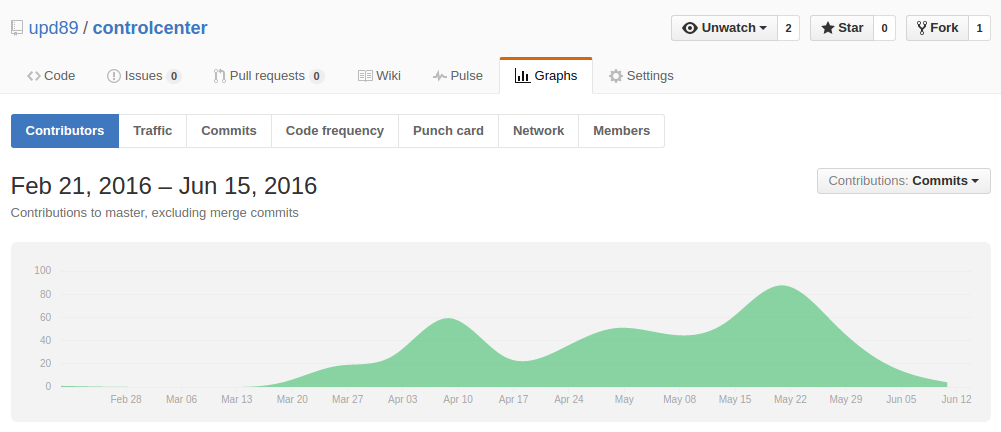
\includegraphics[width=0.95\textwidth]{fig/controlcenter_commits}
  \caption{Anzahl Commits im Control Center}
  \label{fig:commits-cc}
\end{figure}


\begin{figure}
  \centering
    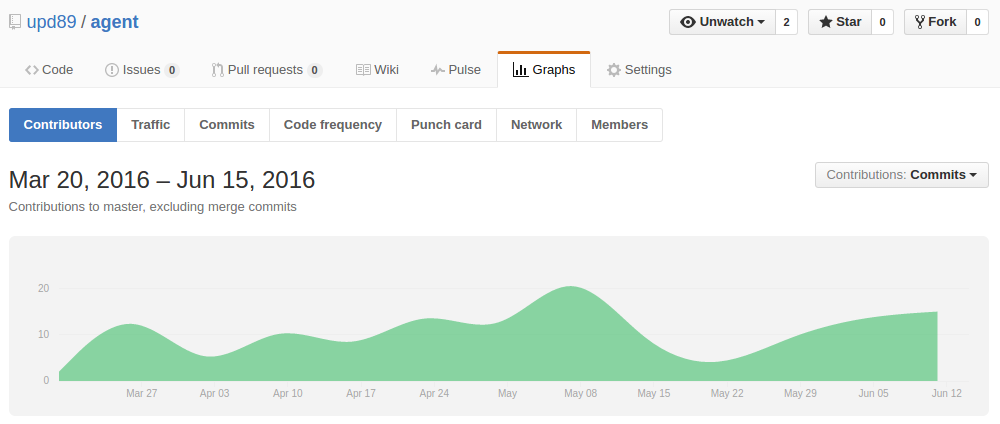
\includegraphics[width=0.95\textwidth]{fig/agent_commits}
  \caption{Anzahl Commits im Agent}
  \label{fig:commits-a}
\end{figure}

Beim Agent (siehe Abbildung \ref{fig:commits-a}) war die Entwicklung mehrheitlich konstant. Lediglich gegen Ende Mai wurden verhältnismässig wenige Änderungen vorgenommen, da beide Teammitglieder vermehrt am Control Center arbeiteten.

Diese Daten können auch über \purl{https://github.com/upd89/controlcenter/graphs/contributors} (Control Center) und \purl{https://github.com/upd89/agent/graphs/contributors} (Agent) direkt eingesehen werden.

\subsection*{Auswertung Redmine}

\subsubsection*{Stunden pro Woche}

Die durchschnittliche Arbeitszeit pro Wochen wurden während dem Semester auf 20 Stunden pro Person festgelegt. Während der Osterwoche wurde dies auf 15 Stunden reduziert. Nach Ende des Semesters und damit der Vorlesungen wurde der geplante Aufwand verdoppelt auf 30-40 Stunden. Für die tabellarische Ansicht siehe Tabelle \ref{tab:phases}.

\begin{table}[H]
    \centering
    \caption{Phasen/Iterationen}
    \label{tab:phases}
    \begin{tabular}{| l | l | l | l | l |}
        \toprule
        Woche & Phase/Iteration & Geplante h pP & Stunden U.B. & Stunden P.C.  \\
        \midrule
        1     & Inception                       & 20   &    18    &  19     \\
        2     & Elaboration 1                   & 20   &    21    &  24.5   \\
        3     & Elaboration 2                   & 20   &    19    &  19     \\
        4     & Elaboration 3                   & 20   &    16.5  &  18.5   \\
        5     & \multirow{2}{*}{Construction 1} & 15   &    14.5  &  19.5   \\
        6     &                                 & 15   &    24    &  14     \\
        7     & \multirow{2}{*}{Construction 2} & 20   &    18    &  19.5   \\
        8     &                                 & 20   &    21.5  &  22.5   \\
        9     & \multirow{2}{*}{Construction 3} & 20   &    20    &  21.5   \\
        10    &                                 & 20   &    22.5  &  22     \\
        11    & \multirow{2}{*}{Construction 4} & 20   &    19.5  &  21     \\
        12    &                                 & 20   &    22    &  20     \\
        13    & \multirow{2}{*}{Construction 5} & 20   &    21    &  19.5   \\
        14    &                                 & 20   &    23.5  &  24     \\
        15    & Transition 1                    & 20   &    21.5  &  23.5   \\
        16    & Transition 2                    & 40   &    43    &  42     \\
        17    & Transition 3                    & 30   &    34    &  33.5   \\
              & Total                           & 360  &    379.5 & 383.5   \\
        \bottomrule
    \end{tabular}
\end{table}

\begin{figure}
  \centering
    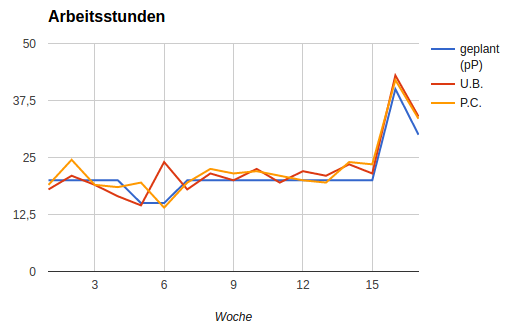
\includegraphics[width=0.8\textwidth]{fig/arbeitsstunden}
  \caption{Auswertung Arbeitsstunden pro Woche}
  \label{fig:workinghours}
\end{figure}

Generell wurden die geplanten Zeiten sehr gut eingehalten (siehe Abbildung \ref{fig:workinghours}). Lediglich in den Osterwochen und am Ende der Construction-Phase wurde mehr Zeit investiert als geplant.

\subsubsection*{Redmine-Tasks}

\begin{figure}
  \centering
    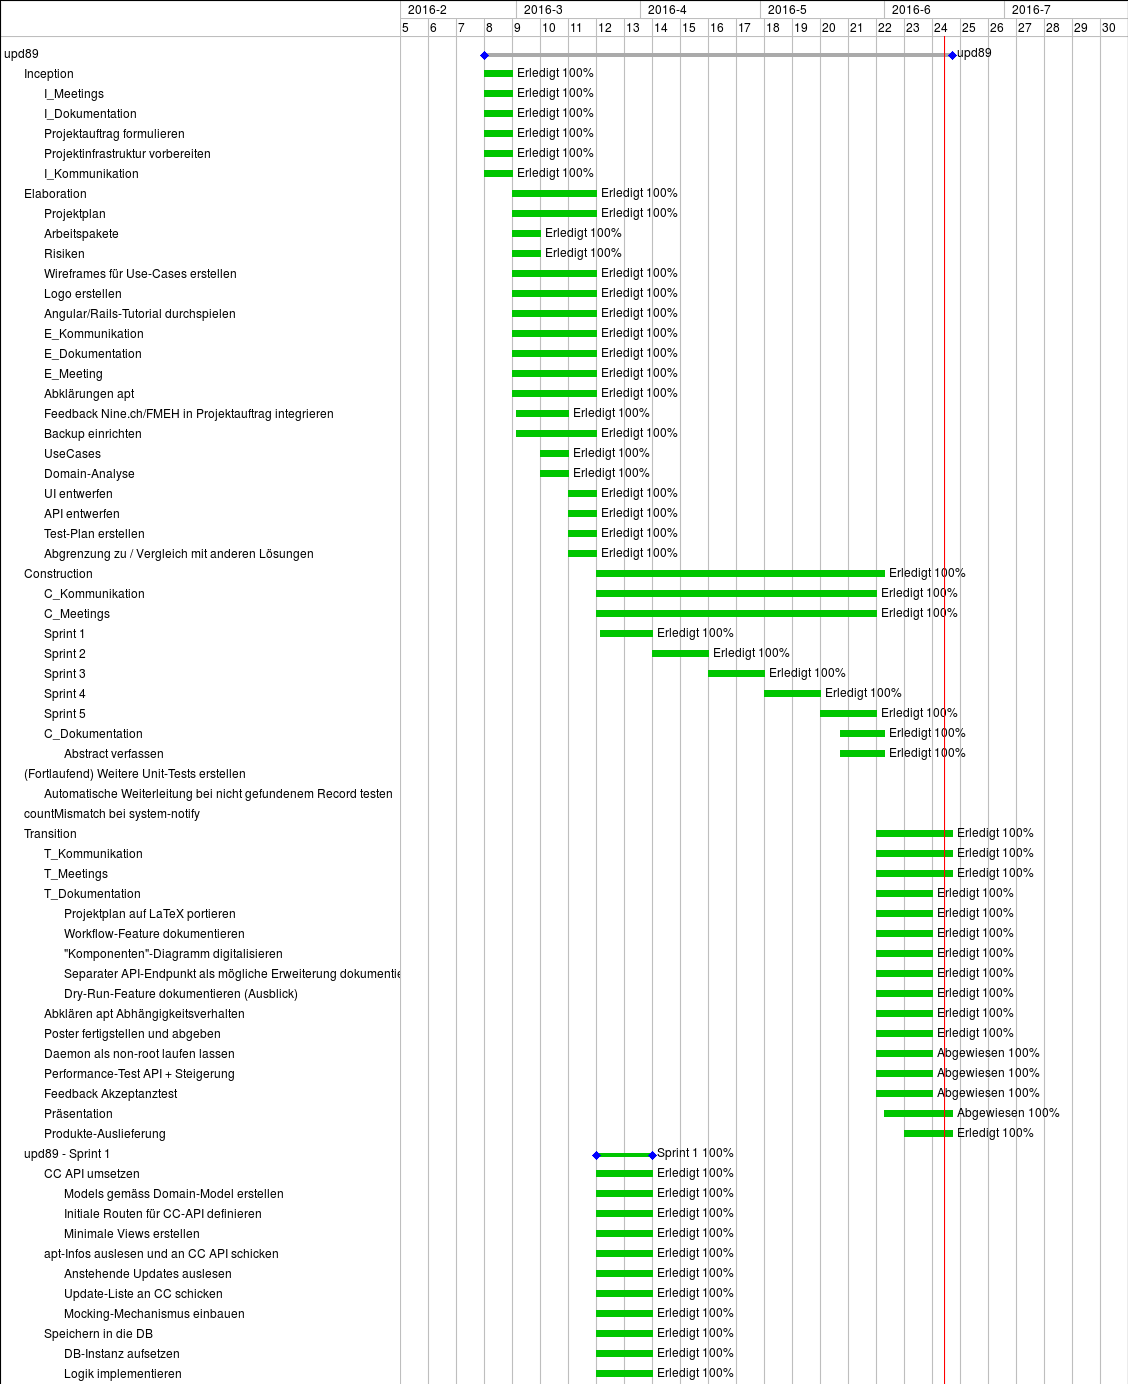
\includegraphics[width=0.95\textwidth]{fig/upd89-gantt-part1}
  \caption{Finales Grantt-Diagram 1/2}
  \label{fig:gantt-final1}
\end{figure}

\begin{figure}
  \centering
    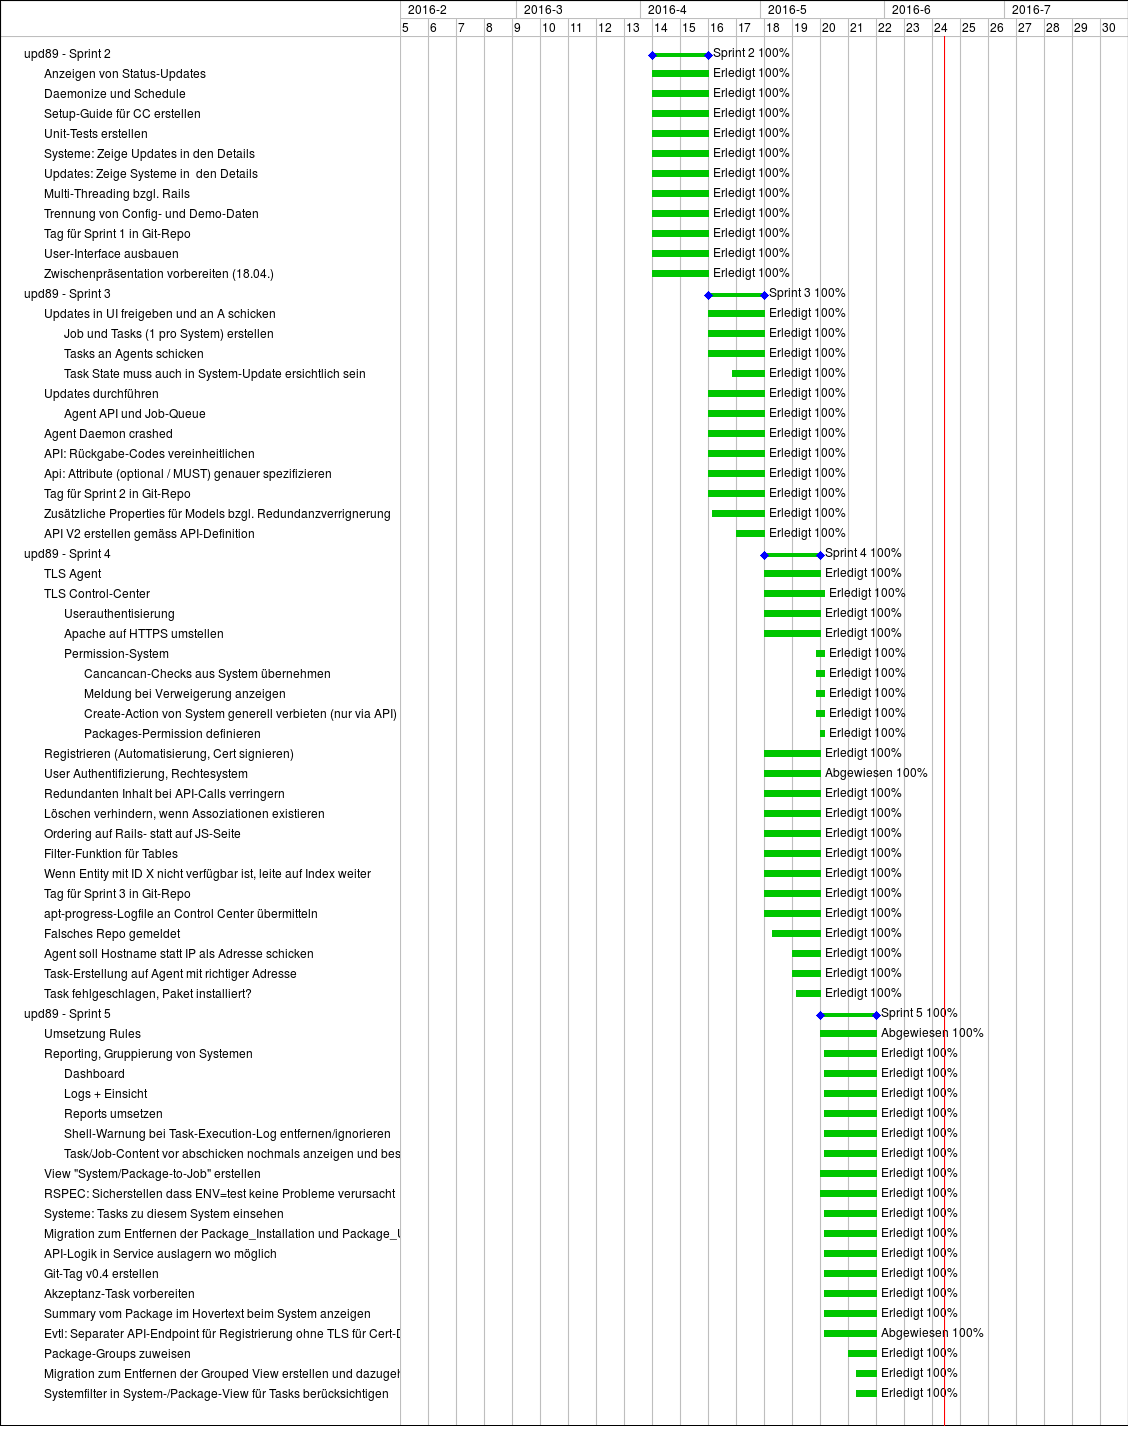
\includegraphics[width=0.95\textwidth]{fig/upd89-gantt-part2}
  \caption{Finales  Grantt-Diagram 2/2}
  \label{fig:gantt-final2}
\end{figure}
